% !TEX root = ../../main.tex
\section{Model Features}\label{sec:method_model_features}
In the previous section we have discussed the \gls{isvdd} method, which creates a \gls{oc-svm} representation of a working set of data objects at every step of the algorithms loop.
This section shows how we interpret the constructed model and extract features to obtain a measure which can be used for an indication of change points.
The next section discusses how this obtained measure is used to indicate change.

The \gls{isvdd} algorithm creates a spherical \gls{oc-svm} representation of the working set at every step of the algorithm.
This model is obtained by the minimization of \Cref{eq:svdd_objective}, which incorporates the radius $R$ of the sphere and the distances $\vectorsym{\xi}$ from the outliers to the boundary.
We will use the radius $R$ of the hypersphere as an indication of change.

In \cite{tax2002uniform} Tax and Duin provide an analysis of the error of the \gls{svdd} algorithm.
This error is based on
\begin{inparaenum}[\itshape 1\upshape)]
\item the fraction $f_{T-}$ of target objects that is rejected, and
\item the fraction $f_{O+}$ of outliers that is accepted.
\end{inparaenum}
Since in \gls{occ} situations typically there are (almost) no examples of outlier objects, Tax and Duin construct a method to generate outliers based on the assumption that the outliers are uniformly distributed around the target set.
To minimize the error, calculated by the fractions $f_{T-}$ and $f_{O+}$, we should minimize the volume of the target data description (\ie the boundary of \gls{svdd}).
That is because the fraction of accepted outliers $f_{O+}$ is an estimate of the volume of the target data description, with respect to the volume of the outlier distribution.
Tax and Duin provide a method to optimize the parameters of the \gls{svdd} method, \ie the trade-off parameter $C$ and the \gls{rbf} kernel width $\sigma$.
This optimization will result in the modification of the radius $R$ of \Cref{eq:svdd_objective} and affects the Lagrangian inequality~(\ref{eq:svdd_inequality}).

\begin{figure}
  \centering
    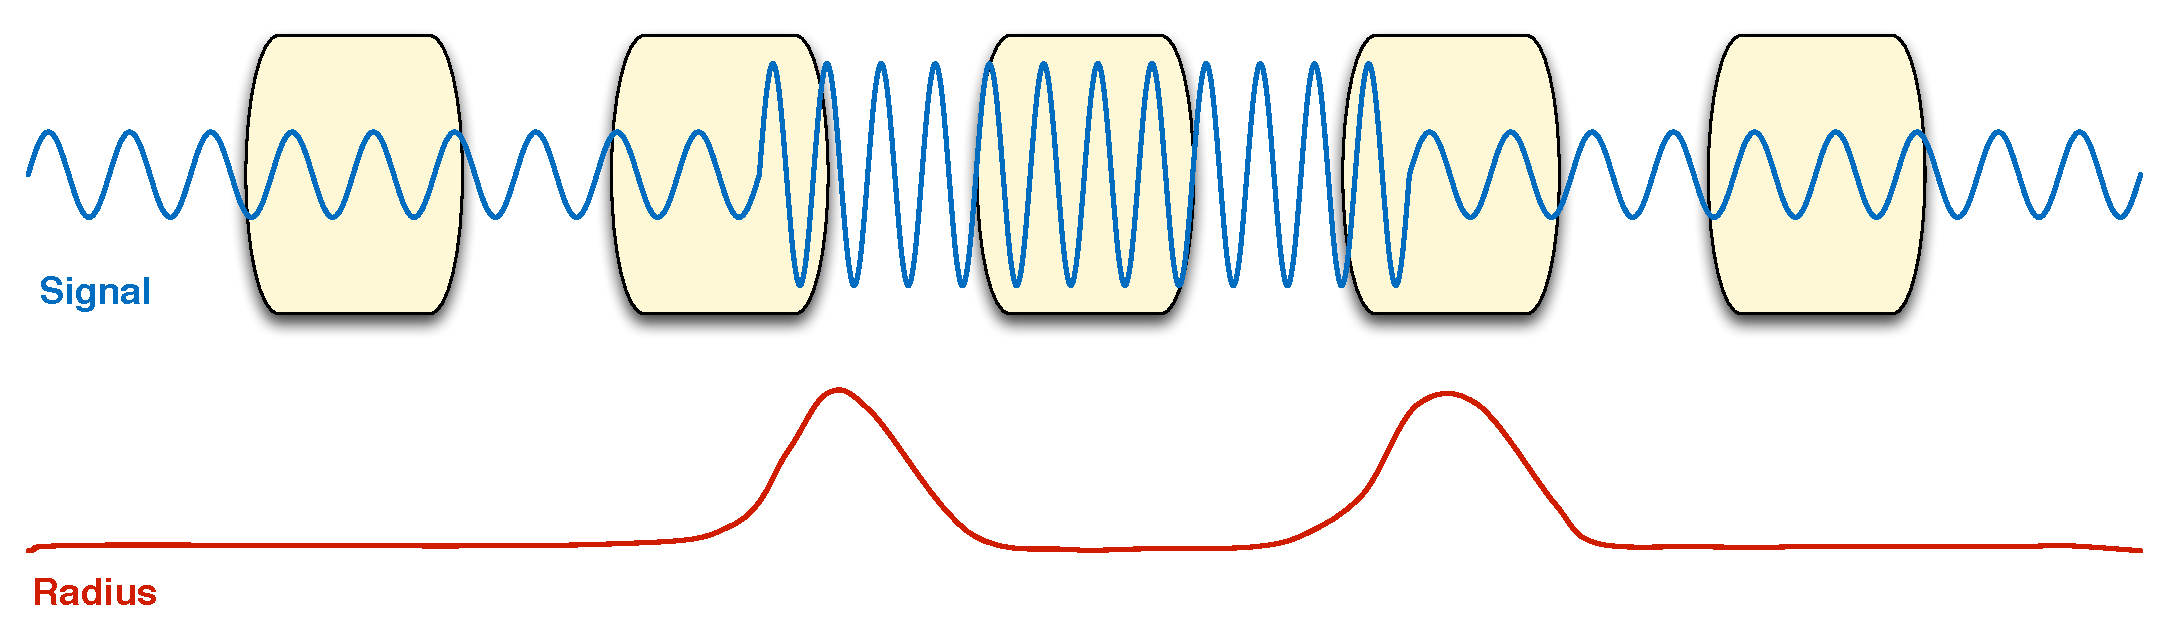
\includegraphics[width=\textwidth,height=\textheight,keepaspectratio]{./Figures/chapter4/expected_behaviour.pdf}
  \caption[Expected radius behavior]{Expected behavior of the radius $R$ of the hypersphere. The upper part shows a typical sinusoidal time series signal. The lower graph visualizes an abstract expectation of the values of $R$. Five possible time windows are illustrated. The left, middle, and right windows cover an area of homogeneous signal. The expected value of $R$ is low. The other two windows cover a change entering and leaving the window, respectively. At these locations the radius $R$ is expected to increase temporarily.}
  \label{fig:radius_expectation}
\end{figure}

Since in our method the parameters $C$ and $\sigma$ are kept constant, and thereby also the fraction of target objects being rejected, the only free parameter is the radius $R$.
During the \gls{isvdd} algorithm the volume of the hypersphere is being minimized.
This means that only the radius of the sphere will change during the analysis over the time series data.
We will interpret changes in the radius $R$ with the same continuity assumptions as mentioned in \Cref{subsec:kernels}.
This means that when two objects (in this case radius sizes) are close to each other, their original objects are also close.
In other words, when the underlying distribution of time series is changed, and thus the characteristics of the data objects changes, the corresponding radius $R$ will also change.
Since in that case the data objects in the working set become more heterogeneous, the radius of the hypersphere will increase.
When, instead, the data objects change from a heterogeneous set to a more homogeneous, we expect the radius to decrease in value, since the data objects are closer to each other in the feature space.
This relation between the signal and expected radius $R$ is illustrated in \Cref{fig:radius_expectation}.
It shows that in the two time windows that cover a heterogeneous set of data objects, the radius of the hypersphere is expected to be relatively high.

With the \gls{isvdd} algorithm we have effectively implemented a form of dimensionality reduction by feature extraction, using the radius $R$.
The following section discusses the algorithms which can be applied to the extracted radius $R$ as a volume estimate.
We thereby follow the setup of the unifying framework by Takeuchi and Yamanishi~\cite{takeuchi2006unifying}, of which this section described the first stage.